As with the circle, we will derive the analytical values for the added mass of an ellipse in motion.
This derivation, unlike the circle, is not straight forward.
And although we will employ the potential of the circle, elliptic coordinates will be introduced to transform this potential so that the ellipse can be studied.
Also unlike the circle, because of its shape, the ellipse will actually have added mass in the sixth mode.


\subsection{Elliptic coordinates}
To study ellipses in the complex plane, we consider the \textsc{\v{Z}ukovsky} transform\footnote{\cite{kennard1967irrotational} \textsc{Kennard}, p.173}
\begin{equation}\label{eq:zukovsky_transform}
  \ezh = \ezh^{\prime} + \frac{c^2}{\ezh^{\prime}}, \qquad \ezh^{\prime} = x^{\prime} + iz^{\prime},
\end{equation}
so that $x^{\prime} = r\cos{\theta}$, $z^{\prime} = r\sin{\theta}$.
Here the prime is no more than a decorator to differentiate the preimage of the \textsc{\v{Z}ukovsky} transform from the complex numbers we will use.
We now have for the complex variable $\ezh = x + iz$, whereupon using \textsc{Euler}'s formula,\footnote{\cite{kennard1967irrotational} \textsc{Kennard}, pp.190--192}
\[
x = \left( r + \frac{c^2}{r} \right)\cos{\theta}, \qquad z =  \left( r - \frac{c^2}{r} \right)\sin{\theta}.
\]
This is indeed an ellipse, as upon squaring both terms and adding them, we get that
\[
\frac{x^2}{a^2} + \frac{z^2}{b^2} = 1, \quad a = r + \frac{c^2}{r}, \quad b = \left\vert r - \frac{c^2}{r} \right\vert.
\]
We call $a$ and  $b$ the major and minor semiaxes, corresponding to the longest and shortest semidiameters of the ellipse, respectively.
The parameter $c = \sqrt{a^2 - b^2}$ is called the focus.
Introducing now the elliptic complex variable $\zeta$, defined by
\[
\ezh^{\prime} = c e^{\zeta}, \qquad \zeta = \xi + i\eta,
\]
where $\xi = \ln{(\sfrac{r}{c})}$ and $\eta = \theta$, we may express the complex number $\ezh$ in terms of this elliptic complex variable such that
\begin{equation}\label{eq:elliptic_ezh}
\ezh = c\cosh{\zeta} = c \big( \cosh{\xi} \cos{\eta} + i \sinh{\xi} \sin{\eta} \big).
\end{equation}
We now clearly see that cricles in $\ezh^{\prime}$ are ellipses in $\ezh$.
Lines of constant $\xi$ constitute confocal ellipses, parametrized with $\eta$, whilst lines of constant $\eta$ are confocal hyperbolas in $\xi$.
We may eliminate either $\xi$ or $\eta$ in equation \eqref{eq:elliptic_ezh} to find that the major and minor semiaxes are respectively given by
\begin{equation}\label{eq:aprime_and_bprime}
a^{\prime} = c\cosh{\xi}, \qquad b^{\prime} = c\absl{\sinh{\xi}}.
\end{equation}
Combining now equations \eqref{eq:elliptic_ezh} and \eqref{eq:aprime_and_bprime},  we find that we may write
\begin{equation}\label{eq:elliptic_xi}
\xi = \ln{\left( \frac{a^{\prime} + b^{\prime}}{c} \right)}, \qquad \xi \geq 0.
\end{equation}
We will use this convention, that $\xi$ be strictly non-negative, though more discussion on this is to be found in \textsc{Kennard}'s work.\footnote{\cite{kennard1967irrotational} \textsc{Kennard} sect.82, pp.192--196}
It is then apparent that the potential for a circle, described in equation \eqref{eq:potential_circle}, may be transformed to give
\begin{equation}\label{eq:potential_ellipse}
w = U\sqrt{\frac{a + b}{a - b}} (b \cos{\alpha} + i a \sin{\alpha}) e^{-\zeta},
\end{equation}
where $\alpha$ is the inclination of the ellipse relative to the direction of motion.
That is, an angle $\alpha = 0$ corresponds to motion along $x$, and $\alpha = \sfrac{\pi}{2}$ corresponds to motion along $z$.
Clearly, by virtue of the above discussion, the real part of the potential is given by
\[
\Phi(\zeta; \alpha) = U \sqrt{\frac{a + b}{a - b}} (b\cos{\alpha} \cos{\eta} + a \sin{\alpha} \sin{\eta}) e^{-\xi},
\]
so that $\phi_1 (\zeta) = \Phi(\zeta; 0)$ and $\phi_2 (\zeta) = \Phi(\zeta; \sfrac{\pi}{2})$.


\subsection{Translatory kinetic energy}
The scale factor of the elliptic coordinate system can be shown to be equal to
\[
h_{\xi} = c\sqrt{\sinh^2{\xi} + \sin^2{\eta}} = \sqrt{{b^{\prime}}^2 + c^2 \sin^2{\eta}}.
\]
Since $q_{\xi} = -{h_{\xi}}^{-1} \partial_{\xi}\Phi = {h_{\xi}}^{-1}\Phi$, and that change in $\xi$ corresponds to a change in $\nhat$, we must have that $q_{\xi} = q_{\nhat}$, where $q_{\nhat} = -{h_{\xi}}^{-1}\partial_{\nhat}\Phi$.
In turn, we have that
\[
q_{\xi} = U \left( \frac{a + b}{a^{\prime} + b^{\prime}} \right) \frac{b \cos{\alpha} \cos{\eta} + a \sin{\alpha} \sin{\eta}}{h_{\xi}}.
\]
Considering the kinetic energy of the fluid, using \textsc{Gauss}' divergence theorem, and using the product rule, we find that
\begin{equation}\label{eq:kinetic_energy_gauss}
T_{\mathrm{fluid}} = \frac{\varrho}{2} \int_{\Omega} q^2 \,\dee V = -\frac{\varrho}{2} \int_{\partial\Omega} \Phi q_{\nhat} \,\dee S.
\end{equation}
Letting $\xi_0$ denote the value of which $\xi$ lies on the ellipse, we assert that such points be represented by $\ezh_0 = a\cos{\eta} + ib\sin{\eta}$.
We then have from equation \eqref{eq:elliptic_xi} that $a^{\prime} = a$ and $b^{\prime} = b$ on the ellipse, and that
\[
\exp{(\xi_0)} = \frac{a + b}{c} = \frac{a + b}{a - b}, \quad \exp{(-\xi_0)} = \frac{a - b}{a + b}.
\]
From the relation that $q_{\nhat} = \partial_s \Psi$,\footnote{\cite{lavrentev1967methoden} \textsc{Lavrentev} \& \textsc{\v{S}abat}, p.233} and that $\dee\Psi = -\partial_{\xi}\Phi\dee\eta$,
\[
T_{\mathrm{fluid}} = \frac{\varrho U^2}{2} \int_{0}^{2\pi} {(b \cos{\alpha} \cos{\eta} + a \sin{\alpha} \sin{\eta})}^2 \,\dee\eta
\]
Calculating the integral, we find that the kinetic energy is given by
\[
T_{\mathrm{fluid}} = \frac{\varrho \pi U^2}{2} (b^2 \cos^2{\alpha} + a^2 \sin^2{\alpha}).
\]
When $a = b$, the ellipse is a circle, and we observe the kintetic energy is what we got for the circle.


\subsection{Rotational kinetic energy}
Consider the complex variable defined as in equation \eqref{eq:elliptic_ezh}, with a potential
\[
w = i A e^{-2\zeta}, \qquad \Psi = Ae^{-2\zeta}\cos{2\eta},
\]
where $A$ is some parameter to be determined.
The stream function satisfies the condition that\footnote{\cite{kennard1967irrotational} \textsc{Kennard}, p.246}
\[
\Psi - \frac{\omega \big( x^2 + z^2 \big)}{2} = C,
\]
where $C$ is some constant.
We recall that $\ezh = x + iz$, so that
\[
A e^{-2\zeta} \cos{2\eta} - \frac{c^2 \omega \big( \cosh{2\xi} + \cos{2\eta} \big)}{4} = C.
\]
We evaluate this at the ellipse $\xi_0$, so that we eliminate $A$ and $\xi$, yielding
\[
w = \frac{i \omega {(a + b)}^2}{4 e^{2\zeta}}, \quad \Phi = \frac{\omega c^2 \sin{2\eta}}{4}.
\]
We may then again use the formulation of the kinetic energy of the fluid as it was presented in equation \eqref{eq:kinetic_energy_gauss}, noting that the differential element $\dee\Psi$ brings with a factor 2, yielding
\[
T_{\mathrm{fluid}} = \frac{\varrho \omega c^4}{16} \int_{0}^{2\pi} \sin^{2}{2\eta} \,\dee\eta = \frac{\pi \varrho \omega c^4}{16}.
\]


\subsection{Added mass}
The added mass can them be found.
\[
\addedmass = \begin{bmatrix}
  \pi\varrho b^2 & 0 & 0\\
  0 & \pi\varrho a^2 & 0\\
  0 & 0 & \sfrac{\pi}{8}\varrho c^4
  \end{bmatrix}
\]


\subsection{Elliptic integrals}
The incomplete elliptic integral of the first kind
\begin{equation}\label{eq:incomplete_elliptic_integral_first}
  \ellF(\phi \vert k) = \int_{0}^{\phi} \frac{1}{\sqrt{1 - k \sin^2{\theta}}}\,\dee\theta
\end{equation}
The complete elliptic integral of the first kind
\begin{equation}\label{eq:complete_elliptic_integral_first}
  \ellK(k) = \ellF(\sfrac{\pi}{2} \vert k) = \int_{0}^{\sfrac{\pi}{2}} \frac{1}{1 - k\sin^2{\theta}} \,\dee\theta
\end{equation}
The incomplete elliptic integral of the second kind
\begin{equation}\label{eq:incomplete_elliptic_integral_second}
  \ellE(\phi \vert k) = \int_{0}^{\phi} \sqrt{1 - k \sin^2{\theta}}\,\dee\theta
\end{equation}


\subsection{The arithmetic-geometric mean}
The arithmetic-geometric mean provides a swift way to calculate elliptic integrals numerically.
Its formulation seems rather arbitrary, but we will quickly see that there is a foundational connection between them.
Further reading is highly encouraged, in particular \emph{Pi and the AGM}\footnote{\cite{borwein1987pi} \textsc{Borwein} \& \textsc{Borwein}} by the \textsc{Borwein} brothers.
Following the literature, we define the arithmetic geometric mean $M$ of $a$ and $b$ through the iterative process
\[
a_{n} = \frac{a_{n-1} + b_{n-1}}{2}, \qquad b_{n} = \sqrt{a_{n-1} b_{n-1}}.
\]
This process is maintained until $c_{n} = \sfrac{1}{2}(a_{n-1} - b_{n-1}) < \epsilon$, where $\epsilon$ is the desired accuracy.
We have assumed that $0 < b_0 \leq a_0$, and we may observe that it is always true that $b_{n-1} \leq b_n \leq a_n \leq a_{n-1}$, so that the values have a common limit.
This limit is the arithmetic-geometric mean:
\[
M(a, b) = \lim_{n \to \infty} a_n = \lim_{n \to \infty} b_n.
\]
It is evident that from this definition, the starting the algorithm at some later iteration must result in the same function.
In other words,
\[
M(a, b) = M{\left( \frac{a + b}{2}, \sqrt{ab} \right)}.
\]
The arithmetic-geometric mean is also obviously homogeneous, meaning $M(\lambda a, \lambda b) = \lambda M(a,b)$, where $\lambda > 0$.
It may be shown that\footnote{\cite{borwein1987pi} \textsc{Borwein} \& \textsc{Borwein}, pp.5--7}
\[
\frac{\pi}{2 M(1, \ezh)} = \int_{0}^{\sfrac{\pi}{2}} \frac{1}{\sqrt{1 - \big( 1 - \ezh^2\big)\sin^2{\theta}}} \,\dee\theta.
\]
A full proof is not appropriately reproduced in this text, so the reader is referred to the \textsc{Borwein} brothers' book.
The relation to elliptic integrals is now quite apparent, in particular
\[
\ellK(k) = \frac{\pi}{2 M(1, k^{\prime})}, \quad \frac{\ellE(k)}{\ellK(k)} = 1 - \sum_{n} 2^{n-1} {c_n}^2.
\]
These are the \texttt{K} and \texttt{E} methods implemented in the \texttt{Jacobi} class of \texttt{jacobi.py}.
At the very heart of these implementations is the descending \textsc{Landen} transform.\footnote{\cite{king1924direct} \textsc{King}, sect.II, IV}
The premise is to start at some modulus $k$ and amplitude $\varphi$, and set
\begin{equation}\label{eq:descending_landen_transform}
k_1 = \frac{1 - k^{\prime}}{1 + k^{\prime}}, \quad \sin{\varphi_1} = \frac{1 + k^{\prime} \sin{\varphi} \cos{\varphi}}{\sqrt{1 - k^2 \sin^2{\varphi}}},
\end{equation}
where $\varphi \leq \varphi_1$.
It can then be shown that
\[
(1 + k^{\prime}) \ellF(\varphi \vert k) = \ellF(\varphi_1 \vert k_1).
\]
Inserting now in equation \eqref{eq:jacobi_dn} that $1 = a^2 \cos^2{\varphi} + b^2 \sin^2{\varphi}$, we get a relationship between the elliptical parameters $a$ and $b$, and the modulus of the elliptic integral, that $k$ is the focus.
Furthermore, it can be shown that equation \eqref{eq:descending_landen_transform} is equivalent to stating that
\[
\sin{( 2\varphi - \varphi_1 )} = k_1 \sin{\varphi_1}.
\]
Through some tedious algebra, we find that this can be written now in terms of an arithmetic-geometric mean algorithm,
\begin{equation}\label{eq:AGM_phi}
\varphi_n = \sfrac{1}{2} \arcsin{\left( \frac{c_{n+1}}{a_{n+1}} \sin{\varphi_{n+1}} \right)} + \frac{\varphi_{n+1}}{2}.
\end{equation}
The above implies that if we run the arithmetic-geometric mean algorithm up until $c_N$ is sufficiently small, we can iterate backwards to find a $\varphi_0$, whence the \emph{descending} \textsc{Landen} transform.
We obviously know what parameters to choose for the arithmetic-geometric mean algorithm, but the starting value of $\varphi_N$ is not as obvious.
It can be shown that the following holds.\footnote{\cite{king1924direct} \textsc{King}, eq.25}
\begin{equation}\label{eq:AGM_ellF}
\ellF(\varphi \vert k) = \frac{\varphi_N}{a_N 2^N}
\end{equation}
This is very handy should we want to calculate any of the \textsc{Jacobi} elliptic functions, since $\ellF$ is the argument.


\subsection{Discretizing the ellipse}
There are multiple ways to approach discretizing the ellipse, the most apparent of which being
\begin{equation}\label{eq:parametric_ellipse}
  \xtt = a\cos{\eta} + ib\sin{\eta}, \qquad \eta \in [0, 2\pi),
\end{equation}
where the parameter $\eta$ is the very same as the elliptic coordinate, called the \emph{eccentric} variable.
It is indeed related, as is clear upon considering $\tan{\eta}$.
This value is equal to $\sfrac{az}{bx}$, by the geometric interpretation of the tangent, where $\xtt = x + iz$.
For a polar representation
\begin{equation}\label{eq:polar_ellipse}
\xtt = r\cos{\theta} + ir\sin{\theta}, \qquad \theta \in [0, 2\pi),
\end{equation}
we find that
\[
\tan{\eta} = \sfrac{a}{b} \tan{\theta}, \quad r(\theta) = \frac{ab}{\sqrt{b^2 \cos^2{\theta} + a^2 \sin^2{\theta}}}.
\]
For the circle, when $a = b$, the eccentric and polar angles are of course equal.
We plot the relationship between the eccentric and polar variables, illustrated in figure \ref{fig:eccentric_versus_polar}.
\begin{Figure}
  \centering
  \scalebox{1}{%
    \begin{tikzpicture}
  \begin{scope}[scale = 2]
    \def\slingringsmonn{.2}
    \def\majorradius{1}
    \def\minorradius{.5}
    \def\miniradius{.1}
    \def\verticaldilation{.5}
    \draw[thick, -latex] (0, {-\verticaldilation*.5*pi-\slingringsmonn})--(0, {\verticaldilation*.5*pi + \slingringsmonn}) node[left]{$\eta$};
    \draw[thick, -latex] ({-(.5*pi+\slingringsmonn)}, 0)--({(.5*pi + \slingringsmonn)}, 0) node[below right]{$\theta$};
    \draw[thick] ({-.5*pi}, .1)--({-.5*pi}, -.1) node[below]{$-\sfrac{\pi}{2}$};
    \draw[thick] ({.5*pi}, .1)--({.5*pi}, -.1) node[below]{$\sfrac{\pi}{2}$};
    \draw[thick] (.1, {-\verticaldilation*(.5*pi)})--(-.1, {-\verticaldilation*(.5*pi)}) node[left]{$-\sfrac{\pi}{2}$};
    \draw[thick] (.1, {\verticaldilation*(.5*pi)})--(-.1, {\verticaldilation*(.5*pi)}) node[left]{$\sfrac{\pi}{2}$};
    \def\smallvalue{.05}
    \draw[domain = {-.5*pi+\smallvalue}:{.5*pi-\smallvalue}, smooth, thick] plot (\x, {\verticaldilation*rad(atan(\majorradius*tan(\x r)/\minorradius))});
    \draw[domain = {-.5*pi+\smallvalue}:{.5*pi-\smallvalue}, smooth, dashed, thick] plot (\x, {\verticaldilation*rad(atan(\majorradius*tan(\x r)/\miniradius))});
  \end{scope}
\end{tikzpicture}

  }
  \captionsetup{type = figure}
  \caption{Relationship between the eccentric variable $\eta$ and polar variable $\theta$. Dashed line is $b = \sfrac{a}{10}$, whole line is $b = \sfrac{a}{2}$.}
  \label{fig:eccentric_versus_polar}
\end{Figure}
We may discretize $\theta$ into a \texttt{linspace}, an array of equally spaced points of the interval $[0, 2\pi)$, and plot the coordinates of the ellipse according to equation \eqref{eq:polar_ellipse}, as is done in figure \ref{fig:polar_ellipse} below.
\begin{Figure}
  \centering
  \scalebox{1}{%
    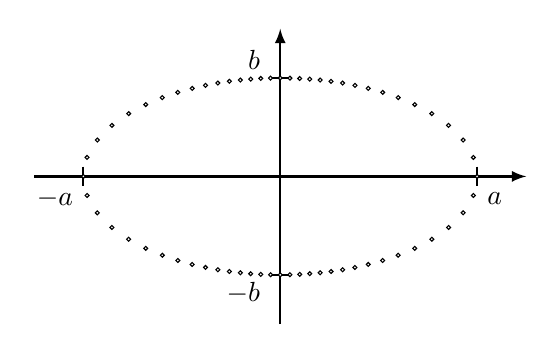
\begin{tikzpicture}
  \begin{scope}[scale = 2.5]
    \def\majradius{1}
    \def\minradius{0.5}
    \def\slingringsmonn{.25}
    \draw[-latex, thick] ({-\majradius - \slingringsmonn}, 0)--({\majradius + \slingringsmonn}, 0);
    \draw[-latex, thick] (0, {-\minradius - \slingringsmonn})--(0, {\minradius + \slingringsmonn});
    \draw[thick] ({-\majradius}, .05)--({-\majradius}, -.05) node[below = 1ex, left]{$-a$};
    \draw[thick] ({\majradius}, .05)--({\majradius}, -.05) node[below = 1ex, right]{$a$};
    \draw[thick] (.05, {\minradius})--(-.05, {\minradius}) node[above = 1.5ex, left]{$b$};
    \draw[thick] (.05, {-\minradius})--(-.05, {-\minradius}) node[below = 1.5ex, left]{$-b$};
    \def\numbernodes{64}
    \foreach \i in {0, ..., \numbernodes}
      \pgfmathsetmacro\teta{2 *\i * pi / \numbernodes}
      \def\radius{(\majradius*\minradius)/sqrt(\minradius^2 * (cos(\teta r))^2 + \majradius^2 * (sin(\teta r))^2)}
      \draw[fill = white] ({\radius*cos(\teta r)}, {\radius*sin(\teta r)}) circle (.01);
  \end{scope}
\end{tikzpicture}

  }
  \captionsetup{type = figure}
  \caption{Ellipse parametrized with the polar variable $\theta$, according to equation \eqref{eq:polar_ellipse}.}
  \label{fig:polar_ellipse}
\end{Figure}
We see that the points tend to accumulate at the top of the ellipse, which indeed makes sense.
As we change the polar angle by an equal amount counter-clockwise, the arc length drawn out between points will diminish towards $\sfrac{\pi}{2}$.
This is illustrated in figure \ref{fig:polar_arc_length_ellipse} below, where points on the ellipse for integer multiples of $\sfrac{\pi}{8}$ are plotted in the first quadrant.
\begin{Figure}
  \centering
  \scalebox{1}{%
    \begin{tikzpicture}
  \begin{scope}[scale = 5]
    \def\slingringsmonn{.2}
    \def\majorradius{1}
    \def\minorradius{.5}
    \draw[thick, -latex] ({-\slingringsmonn}, 0)--({\majorradius + \slingringsmonn}, 0);
    \draw[thick, -latex] (0, {-\slingringsmonn})--(0, {\minorradius + \slingringsmonn});
    \draw[thick] (\majorradius, .05)--(\majorradius, -.05) node[below]{$a$};
    \draw[thick] (.05, \minorradius)--(-.05, \minorradius) node[left]{$b$};
    \foreach \i in {0, ..., 4}
      \pgfmathsetmacro\teta{\i * pi / 8}
      \def\radius{(\majorradius*\minorradius)/sqrt(\minorradius^2 * (cos(\teta r))^2 + \majorradius^2 * (sin(\teta r))^2)}
      \draw[fill = white] ({\radius*cos(\teta r)}, {\radius*sin(\teta r)}) circle (.01);
  \end{scope}
\end{tikzpicture}

  }
  \captionsetup{type = figure}
  \caption{Demonstration that the arc length between points decreases counter-clockwise in the first quadrant as the polar angle $\theta$ approaches $\sfrac{\pi}{2}$.}
  \label{fig:polar_arc_length_ellipse}
\end{Figure}
This is not the case for the ellipse discretized according to equation \eqref{eq:parametric_ellipse}, using the eccentric variable $\eta$, as is seen in figure \ref{fig:eccentric_ellipse} below.
\begin{Figure}
  \centering
  \scalebox{1}{%
    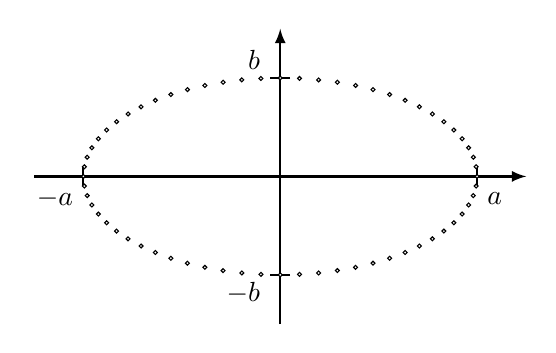
\begin{tikzpicture}
  \begin{scope}[scale = 2.5]
    \def\majradius{1}
    \def\minradius{.5}
    \def\slingringsmonn{.25}
    \draw[-latex, thick] ({-\majradius - \slingringsmonn}, 0)--({\majradius + \slingringsmonn}, 0);
    \draw[-latex, thick] (0, {-\minradius - \slingringsmonn})--(0, {\minradius + \slingringsmonn});
    \draw[thick] ({-\majradius}, .05)--({-\majradius}, -.05) node[below = 1ex, left]{$-a$};
    \draw[thick] ({\majradius}, .05)--({\majradius}, -.05) node[below = 1ex, right]{$a$};
    \draw[thick] (.05, {\minradius})--(-.05, {\minradius}) node[above = 1.5ex, left]{$b$};
    \draw[thick] (.05, {-\minradius})--(-.05, {-\minradius}) node[below = 1.5ex, left]{$-b$};
    \def\numbernodes{64}
    \foreach \i in {1, ..., \numbernodes}
      \draw[fill = white] ({\majradius*cos(2*\i*pi/\numbernodes r)}, {\minradius*sin(2*\i*pi/\numbernodes r)}) circle (.01);
  \end{scope}
\end{tikzpicture}

  }
  \captionsetup{type = figure}
  \caption{Ellipse parametrized with the eccentric variable $\eta$, according to equation \eqref{eq:parametric_ellipse}.}
  \label{fig:eccentric_ellipse}
\end{Figure}
\begin{Figure}
  \centering
  \scalebox{1}{%
    \begin{tikzpicture}
  \begin{scope}[scale = 5]
    \def\slingringsmonn{.2}
    \def\majorradius{1}
    \def\minorradius{.5}
    \draw[thick, -latex] ({-\slingringsmonn}, 0)--({\majorradius + \slingringsmonn}, 0);
    \draw[thick, -latex] (0, {-\slingringsmonn})--(0, {\minorradius + \slingringsmonn});
    \draw[thick] (\majorradius, .05)--(\majorradius, -.05) node[below]{$a$};
    \draw[thick] (.05, \minorradius)--(-.05, \minorradius) node[left]{$b$};
    \foreach \i in {0, ..., 4}
      \pgfmathsetmacro\teta{\i * pi / 8}
      \draw[fill = white] ({\majorradius*cos(\teta r)}, {\minorradius*sin(\teta r)}) circle (.01);
  \end{scope}
\end{tikzpicture}

  }
  \captionsetup{type = figure}
  \caption{Arc length increases counter-clockwise in the first quadrant as the eccentric variable $\eta$ approaches $\sfrac{\pi}{2}$.}
\end{Figure}
Of interest to investigate is how these distributions of nodes impact the convergence of the software---one thought is that performance of tendency for nodes to concentrate towards either of the semiaxes will positively impact the accuracy for the corresponding mode.
To be investigated is also whether a distribution such that arc lengths between nodes remain constant over the whole ellipse will perform better than either the eccentric or polar representation.

